\documentclass[article,oneside]{memoir}

\usepackage{amsmath}
\usepackage{amssymb}
\usepackage{cclicenses}
\usepackage{color}
\usepackage{euler}
\usepackage[colorlinks=true,linkcolor=blue,citecolor=red]{hyperref}
\usepackage{float}
\usepackage{framed}
\usepackage[letterpaper,margin=2.5cm]{geometry}
\usepackage{graphicx}
\usepackage{indentfirst}
\usepackage{longtable}
\usepackage[final]{microtype}
\usepackage{multicol}
\usepackage{nameref}
\usepackage{pdflscape}
\usepackage{pdfpages}
\usepackage{tabularx}
\usepackage{textcomp}
\usepackage{todonotes}
\usepackage{libertine}
\usepackage{inconsolata}


% PAGE SETUP
\setlength{\parindent}{5mm}
\nonzeroparskip
\raggedbottom
\raggedcolumns

% CONFIG FOR TOC, BIBLIO, ETC
\setcounter{tocdepth}{2}
\renewcommand{\bibname}{References}

% HANDY DEFINITIONS
\newcommand{\note}[1]{ \begin{framed} #1 \end{framed} }
\newcommand{\refdes}[1]{\texttt{#1}}
\newcommand{\mr}[1]{\ensuremath{\mathrm{#1}}}
\newcommand{\schematicpage}[2]{ \begin{framed} Relevant schematic page: \hyperlink{schematic.pdf.#1}{\texttt{#2/#1}} \end{framed} }

\title{Owner's Manual}
\author{WCP52}

\begin{document}

\pagestyle{headings}
\begin{titlingpage}
%\setlength\extrarowheight{10mm}
\begin{tabularx}{\textwidth}{Xr}
\hline
\\
{\LARGE OWNER'S AND SERVICE MANUAL} &
Gain/Phase Analyzer \\
\\
\hline
\end{tabularx}
\vfill
\begin{center}
\missingfigure[figwidth=4in]{Photo}
\end{center}
\vfill
\begin{center}
\textcopyright 2015, WCP52. Licensed under a Creative Commons Attribution 4.0 International License.
\end{center}
\end{titlingpage}

\begin{multicols}{2}

\tableofcontents
\listoffigures

\newpage
\chapter{Introduction}
\label{chap:intro}


\newpage
\chapter{Specifications}


\newpage
\chapter{Operating Information}


\newpage
\end{multicols}
\newpage
\begin{figure}[h]
\centering
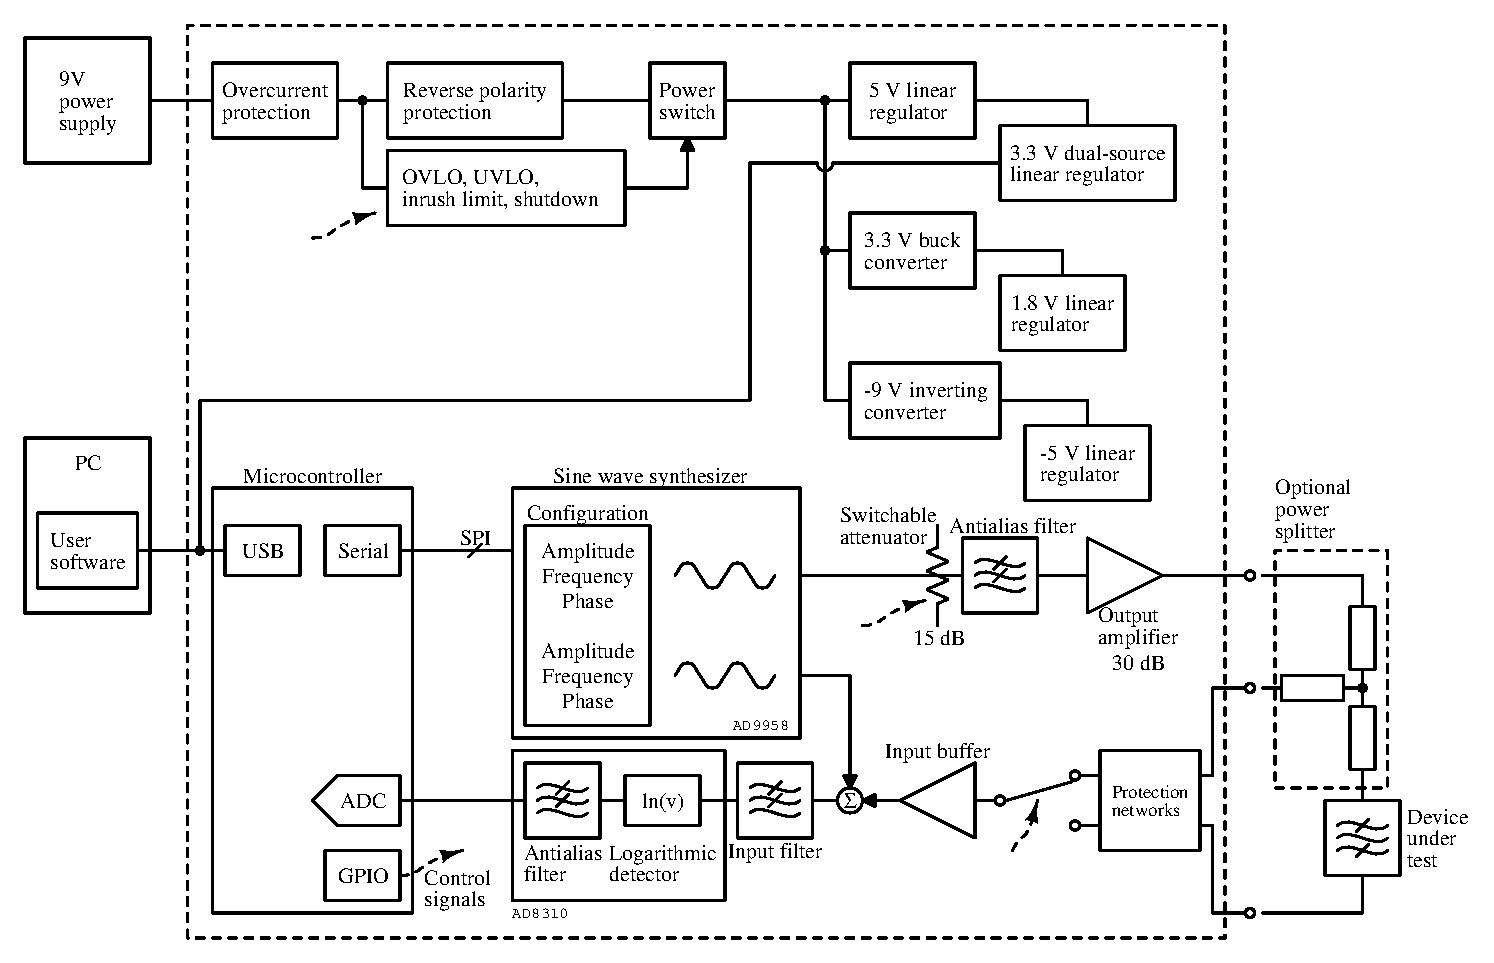
\includegraphics[width=6.5in]{blockdiagram}
\caption{Block diagram}
\label{fig:blockdiagram}
\end{figure}
\begin{multicols}{2}

\chapter{Theory of Operation}

This section contains a decription of the operation of the gain/phase analyzer.
Explanations range from simple and broad to very specific.
It is expected that the reader has an understanding of the basics of
gain/phase analysis itself, which is explained in the \hyperref[chap:intro]{Introduction
chapter}.

Also, it will be beneficial to look at the main system schematics when reading
through this section. Small pieces of the schematic are excerpted when helpful
in explaining their function, but are not always shown.

\section{Block Description}

The block diagram is shown in figure~\ref{fig:blockdiagram}. A microcontroller
drives the instrument, configuring a dual sine wave synthesizer via a serial
interface.  The first output passes through an optional, switchable attenuator,
allowing output amplitude to be configured beyond the practical amplitude range
of the synthesizer. The signal is then filtered to attenuate Nyquist aliasing,
and then amplified by $30\;\mr{dB}$ before being passed to the output.

Signals returning from the Device Under Test (DUT) pass through input protection
networks, then enter a double-throw RF switch allowing one of them to be
analyzed. An input buffer prevents signals from further circuitry from feeding
back out the input and affecting the DUT. A summing network combines the input
signal with the second output of the synthesizer, and the sum passes through an
input filter and into a logarithmic detector. The logarithmic detector outputs a
voltage corresponding to the signal amplitude in decibels, and this is further
filtered to allow slow sampling, and returns to the microcontroller via the
on-chip analog to digital converter.

A power supply system provides overcurrent protection, reverse polarity
protection, overvoltage lockout, undervoltage lockout, inrush limiting, and
microcontroller-driven shutdown (used in cases of USB suspend). It produces
regulated voltage rails of $+9\;\mr{V}$ and $-9\;\mr{V}$ (for the final output
amplifier stage), $+5\;\mr{V}$ and $-5\;\mr{V}$ (for general linear circuitry),
$+3.3\;\mr{V}$ (for the synthesizer), $+1.8\;\mr{V}$ (for the synthesizer),
and a second, weaker $+3.3\;\mr{V}$ rail that can be powered by the USB port in
the absence of the main power input (for the microcontroller).

A USB interface connects to a computer, where software sends control commands to
the instrument and plots received data.


\section{Detailed Circuit Description}
\subsection{Power Input Circuit}

This instrument is complex and has many somewhat expensive parts, so a full
input subsystem was designed to ensure that these parts are always supplied
correctly with power. This subsystem provides the following features:

\begin{itemize}
\item{Overcurrent protection}
\item{Reverse polarity protection}
\item{Undervoltage lockout}
\item{Overvoltage protection}
\item{Inrush current limiting}
\end{itemize}

\subsubsection{Overcurrent protection}

The first piece of this input system, and possibly the simplest, is
\refdes{R81}. \refdes{R81} is a \emph{resettable fuse}, a type of resistor
with a positive temperature coefficient. Its resistance is very low
(around $0.5\;\Omega$) at room temperature.  As the current flowing through it
increases, it heats up, and as it heats up, its resistance increases.
Eventually, it will reach a point where this process `snowballs', and its
resistance is high enough that almost no current can flow through it. This
allows it to act like a fuse, but without permanently blowing: as soon as it
cools back down, it will conduct again.

\begin{figure}[H]
\centering
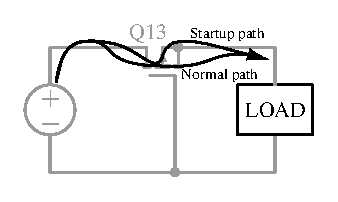
\includegraphics[width=3in]{mosrpp}
\caption{MOS reverse polarity protection circuit, simplified}
\label{fig:mosrpp}
\end{figure}

\subsubsection{Reverse polarity protection}

Once input current has passed through the resettable fuse, it encounters
\refdes{Q13}. A simplified form of this part of the circuit can be seen in
figure~\ref{fig:mosrpp}. Remember that a MOSFET has `parasitic' diodes
connected from the transistor's channel to its substrate; in a
standard power MOSFET, one ends up connected between the two ends of the
channel (the other ends up shorted to itself). In a P-channel MOSFET, this
diode points from the source to the drain. In this circuit, when power is
applied with the correct polarity, this diode allows current to initially take
the path labeled \emph{startup path}. When it does so, the voltage applied to
the load begins to rise, but the gate stays low, as it is tied to ground.
Eventually, the voltage rises high enough that the gate-source voltage switches
on the MOSFET, and current begins to flow through the \emph{normal path}
instead. This path takes the current through the low-impedance MOSFET channel,
rather than through the diode where the forward threshold voltage of the diode
would be lost.

If power is applied in the incorrect polarity, the substrate diode never
conducts, so the MOSFET never switches on.

\subsubsection{Power switch}

After the reverse polarity protection, the current must flow through
\refdes{Q14}, which is connected as a traditional switch. \refdes{R88} holds
its gate and source together when the power is switched off, keeping the MOSFET
also turned off.

%\end{multicols}
\begin{figure}[H]
\centering
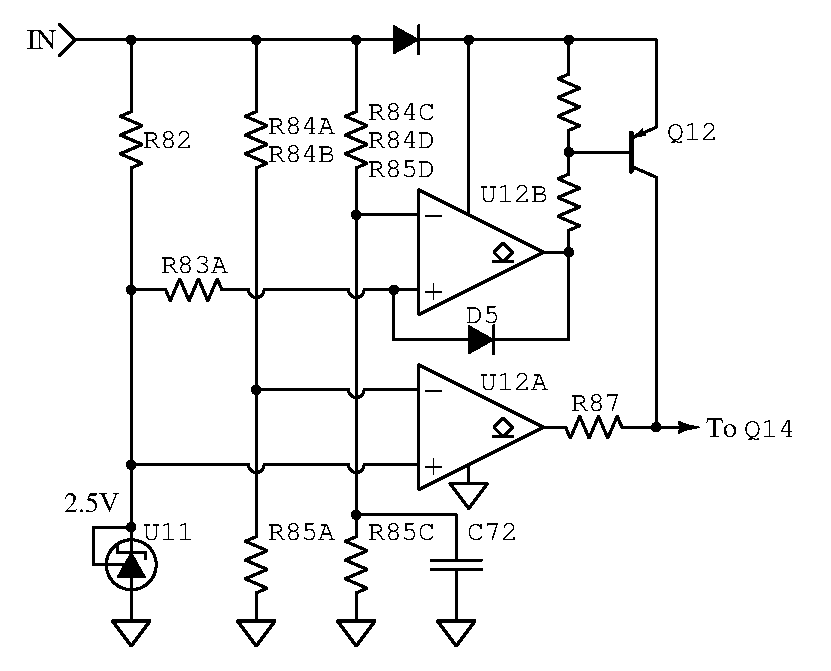
\includegraphics[width=3in]{comparator}
\caption{UVLO and OVLO circuit}
\label{fig:uovlo}
\end{figure}
%\begin{multicols}{2}

To simplify things, the subcircuit in figure~\ref{fig:uovlo} is powered through
a single diode for its own reverse-polarity protection. Bandgap voltage reference
\refdes{U11} does not need this, as its internal circuit has an antiparallel diode
built in~\cite{tl431}.

\subsubsection{Undervoltage lockout}

\refdes{U11} provides an accurate $2.5\;\mr{V}$ level against which the input
voltage can be compared. As the input voltage rises, the voltage at the output of
the \refdes{R84A}/\refdes{R84B}/\refdes{R85A} voltage divider also rises. When
this divided voltage reaches the $2.5\;\mr{V}$ reference level, the input voltage
is at $7.5\;\mr{V}$, the undervoltage threshold. Comparator \refdes{U12A}
switches low, allowing power switch \refdes{Q14} to switch on and allow the
full system to operate.

\subsubsection{Overvoltage protection}

If the input voltage continues to rise, the voltage at the output of the
\refdes{R84C}/\refdes{R84D}/\refdes{R85D}/\refdes{R85C} voltage divider will
eventually reach the reference level when the input voltage is at $10\;\mr{V}$.
\refdes{C72} provides a low-pass effect which prevents simple noise and short
transients from causing this. When this happens, comparator \refdes{U12B}
switches low. At this point, two things happen. First, \refdes{Q12} switches
\refdes{Q14} off, powering down the circuit. Second, \refdes{D5} pulls the
reference level as seen by \refdes{U12B} down to about $1\;\mr{V}$, locking
the system in this shutdown mode until the input voltage drops back as low
as $4\;\mr{V}$ --- at which point it must climb again to the $7.5\;\mr{V}$
undervoltage threshold. In practice, the system must be powered off and back
on. This latch prevents the instrument from accidentally being powered by
too high an input voltage.

\subsubsection{Inrush current limiting}

\refdes{Q14} does not act \emph{only} as a power switch. When it switches on,
it starts in the `cutoff' region of operation, and moves to the `saturation'
region. However, it must pass through the `linear' region. We can take
advantage of this.

\begin{figure}[H]
\centering
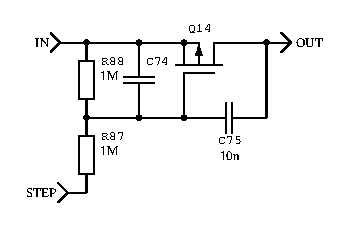
\includegraphics[width=3in]{millerint}
\caption{Miller integrator}
\label{fig:miller}
\end{figure}

The circuit in figure~\ref{fig:miller}, when \refdes{Q14} is in the linear
region, is known as a `Miller integrator'~\cite[pg. 283]{tranckts-sawtooth}.
Because \texttt{R87} and \texttt{R88} form a voltage divider, the input
voltage to the integrator will be half the input supply voltage at half
the resistance (nominally, $4.5\;\mr{V}$ at $500\;\mr{k\Omega}$). The
integrator capacitance is simply \texttt{C75}, which is $10\;\mr{nF}$.
Because the voltage across \texttt{C74} changes only negligibly, its effect
on the circuit will also be negligible.

At startup, \refdes{C75} would tend to hold the gate above the source,
switching the transistor fully on and bypassing any limiting effect. The
much larger \refdes{C74} swamps this effect, holding the gate to the
source until a DC source of current is provided via \refdes{R87}.

The input signal to this integrator will be a step, because comparator
\texttt{U12A} switches directly from `off' to `on'. Integrating a step gives
a ramp, with a slope of:

\begin{equation*}
    \frac{dv}{dt} = \frac{v_\mr{in}}{RC} = \frac{4.5\;\mr{V}}{(500\;\mr{k\Omega})(10\;\mr{nF})}
    = 900\;\mr{V/s} = 0.9\;\mr{V/ms}
\end{equation*}

This means it will take about $10\;\mr{ms}$ for the voltage to ramp from zero
to the full input voltage of $9\;\mr{V}$.

Because the inrush current to be limited is the current charging the system's
capacitance, we can calculate the worst-case inrush current. Charge is held
on-board by approximately $200\;\mr{\mu F}$ worth of capacitors. Given this
capacitance and the voltage slope, the current is calculated as follows:

\begin{equation*}
    I = C \frac{dv}{dt} = (200\;\mr{\mu F})(900\;\mr{V/s}) = 180\;\mr{mA}
\end{equation*}

During this charging time, the power dissipated in \texttt{Q14} will be high.
The worst-case is when the full input voltage is dropped across it, giving
a power dissipation of $(9\;\mr{V})(180\;\mr{mA}) = 1.62\;\mr{W}$. The average
power for the entire time will be:

\begin{gather*}
    P = IV \\
    P_\mr{avg} = \frac{1}{10\;\mr{ms}}\int_0^{10ms} iv\;dt \\
    {}= \tfrac{1}{2}(1.62\;\mr{W})(10\;\mr{ms})/(10\;\mr{ms}) \\
    {}= 810\;\mr{mW} \\
\end{gather*}

Thus, a MOSFET must be selected that can handle an $810\;\mr{mW}$ pulse for
$10\;\mr{ms}$. This pulse-handling capability is shown in the datasheet as
the ``forward-biased safe operating area'', and we selected an AOD417 which
can easily handle this pulse with excess~\cite{aod417}.

\begin{figure}[H]
\centering
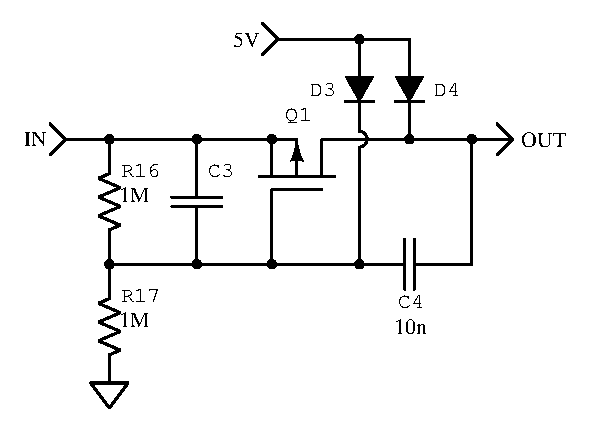
\includegraphics[width=3in]{usbinput}
\caption{USB power input circuit}
\label{fig:usbpower}
\end{figure}

\subsubsection{USB Power Input Circuit}

The USB specification is very demanding with respect to the amount of inrush
current that a USB device may consume. We used the same Miller-integrator
inrush limiting circuit on the USB power supply input.

In this case, the resistance has not changed (still a Th\'evenin-equivalent
$500\;\mr{k\Omega}$), and the input step is equal to $2.5\;\mr{V}$, half the
input voltage. The integrating capacitance is \refdes{C4}, which has a value of $10\;\mr{nF}$,
and the maximum input capacitance being charged is approximately $20\;\mr{\mu F}$.

\begin{gather*}
    \frac{dv}{dt} = \frac{v_\mr{in}}{RC} = \frac{2.5\;\mr{V}}{(500\;\mr{k\Omega})(10\;\mr{nF})}
    = 500\;\mr{V/s} \\
    I = C \frac{dv}{dt} = (20\;\mr{\mu F})(500\;\mr{V/s}) = 10\;\mr{mA}
\end{gather*}

The power dissipation in this case is very small (no more than $50\;\mr{mW}$ for
only a few milliseconds), so we used a smaller and less expensive MOSFET that
was already in use elsewhere for this particular integrator.

No reverse polarity protection was deemed necessary on the USB input.

Diodes \refdes{D3} and \refdes{D4} allow the on-board power supply to power
the circuitry downstream from the USB port whenever that supply is powered,
so that this circuitry can draw larger amounts of current without the trouble
of making sure that this current draw is within USB specifications.
\refdes{D3} shuts off \refdes{Q1}, and \refdes{D4} provides power in
\refdes{Q1}'s absence.


\subsection{Switching DC-DC Converters}

\begin{figure}[H]
\centering
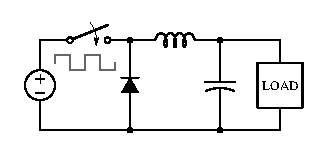
\includegraphics[width=3in]{buckconv}
\caption{Basic buck converter circuit}
\label{fig:basicbuck}
\end{figure}

\subsubsection{Buck converter theory}

The basic idea of an inductor is that it translates electric current flowing
through it into a magnetic field around it. There is energy stored in this
magnetic field, so the inductor tends to hold the current fixed (as changing
the current would require adding or removing energy from the field). The
`buck converter' is a voltage down-converter circuit that takes advantage
of this.

A more mathematical approach is that inductors integrate the voltage applied
to them, producing a current:

\begin{equation*}
    i = \frac{1}{L} \int v\;dt
\end{equation*}

A buck converter must have at least one switch, as shown in
figure~\ref{fig:basicbuck}.  The switch is initially closed for a brief period.
This applies a positive voltage to the inductor, causing the current through it
to begin to increase (remember that the integral of a step is a ramp). This
current flows through to the output of the converter, and the output voltage
begins to rise.

Now, the switch is opened. The inductor keeps the current flowing, though,
through the diode this time. The voltage across the inductor is now negative
(the voltage on the left side had to fall negative in order to forward-bias the
diode and make it conduct), so the current starts ramping downward, and the
output voltage begins to fall.~\cite[pp.~356--357]{aoe-vreg}

By repeating this cycle, the output voltage can be made to rise and fall around
a desired point, and by placing a large capacitor at the output, the rising and
falling current can translate to very small variation in output voltage, though
it must rise and fall at least a small amount. This allows the output voltage
to be any arbitrary voltage smaller than the input voltage, but does not
theoretically lose power, unlike a linear regulator (whose entire mechanism of
operation is intentional power loss).


\begin{figure}[H]
\centering
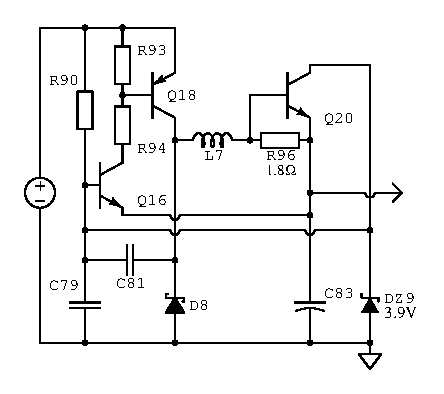
\includegraphics[width=3in]{3v3buck}
\caption{$3.3\;\mr{V}$ buck converter circuit}
\label{fig:3v3buck}
\end{figure}

\subsubsection{3.3 V buck converter}

In this instrument, we have used a simple, three-transistor regulated buck
converter circuit. It is inexpensive, reliable, and though it is not hugely
efficient, it generates relatively little switching noise (due, in part, to
its low speed compared to more modern designs).

In the first phase of the switching cycle, \refdes{Q16}'s base voltage is
low. \refdes{R90} charges \refdes{C79}, and eventually the base voltage rises
high enough that \refdes{Q16} switches on. It pulls \refdes{Q18}'s base voltage
down, switching on that transistor too. \refdes{Q18} is equivalent to the main
switch in figure~\ref{fig:basicbuck}, and the inductor current starts to rise.

In the next phase of the switching cycle, something draws current towards ground
out of \refdes{C79} and away from \refdes{Q16}'s base. This starts a chain reaction:
\refdes{Q16} and \refdes{Q18} start to switch off, and are no longer driving the
inductor. The inductor's tendency to keep current flowing makes the voltage on its
left side sharply decrease. This decrease is coupled through \refdes{C81}, which
drags \refdes{Q16}'s base voltage even lower, switching it off quite solidly.
The converter will remain switched off until \refdes{C79} charges back up through
its resistor.

Two things can be the `something' of the previous paragraph, initiating the
switch from phase 1 to phase 2. First, note that \refdes{Q16}'s emitter is
connected to the output voltage, so when it is switched on, its base will be
about $0.65\;\mr{V}$ above that. When the output voltage reaches about
$3.25\;\mr{V}$, the base voltage is at about $3.9\;\mr{V}$, and Zener diode
\refdes{DZ9} starts to conduct. This means that the output voltage will not be
allowed to rise above about $3.25\;\mr{V}$, providing the voltage regulation
function.

The inductor current must also flow through sense resistor \refdes{R96}. If the
current exceeds about $650\;\mr{mA}$, the base-emitter voltage applied to
\refdes{Q20} will be high enough to switch it on, and \refdes{Q20} will draw the
shutdown current. This provides the current-limiting function.

\subsubsection{-9V inverting regulator}
It is possible to repurpose a buck converter circuit as an inverting
(buck-boost) circuit that generates a negative voltage~\cite{buckinv}. The
circuit is otherwise the same, with two exceptions. First, the Zener diode, now
\refdes{DZ10}, is a $10\;\mr{V}$ part, giving a regulated output voltage of
about $9.35\;\mr{V}$. Second, because the current through the output capacitor
has more hard edges in a buck-boost converter, a $1\;\mr{\mu F}$ ceramic
capacitor (useful to higher frequencies and currents) has been added in
parallel with the main output capacitor.

\subsection{Linear Regulators}
A series-type linear regulator works by acting as a controlled resistance,
regulating itself to exactly the resistance required to give the correct
output voltage considering the amount of current flowing through it. This
means that power loss is a required property of linear regulators. For example,
a linear regulator taking an input voltage of $9\;\mr{V}$, giving an output
voltage of $5\;\mr{V}$, and passing a current of $100\;\mr{mA}$, will
lose $(9-5)(0.1)\;\mr{W} = 400\;\mr{mW}$ of power, dissipated as heat.
The loss is sometimes a fair trade for simplicity and low output noise.
This instrument uses four linear regulators, which provide power supplies
of $5\;\mr{V}$, $-5\;\mr{V}$, $1.8\;\mr{V}$, and a low-power $3.3\;\mr{V}$
supply (a high-power $3.3\;\mr{V}$ supply for the synthesizer comes from
the buck converter).

These regulators are \refdes{U13}, \refdes{U14}, \refdes{U15}, and \refdes{U16}.
They are monolithic devices with no external circuitry except for filter
capacitors, and as such will not be addressed further. See their datasheets for
more information:~\cite{l78m05}~\cite{mc79m00}~\cite{az1117c}~\cite{mcp1700}.

\subsection{Microcontroller}
\subsubsection{USB Communications}

\subsection{Synthesizer}

\subsection{Synthesizer Output Amplifiers}

\subsection{Output System}

\subsubsection{Attenuator and Filter}
\subsubsection{Gain Stages and Termination}

\subsection{Input System}

\subsubsection{Protection}
\subsubsection{Switching}

It would not be practical for the analyzer to contain two independent input
subsystems to measure both inputs, as these systems are complex and expensive,
and there would be significant variation between the two. Instead, one input
subsystem is switched between two inputs. This switching is accomplished with a
pair of high-bandwidth SPST RF analog switches.

\begin{figure}[H]
\centering
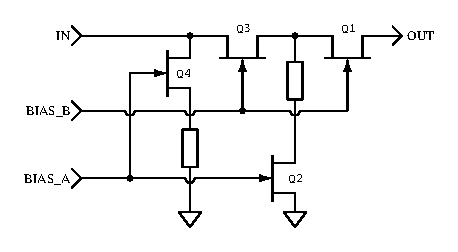
\includegraphics{gaassw}
\caption{GaAs switch circuit}
\label{fig:gaassw}
\end{figure}

Figure~\ref{fig:gaassw} shows the internal circuit of the
switch~\cite{maswss0162}.  It is a simple circuit built from four gallium
arsenide (GaAs) FETs \footnote{The type of FET used is a relatively uncommon
    variant called a \emph{MESFET}, or MEtal-Semiconductor Field Effect
Transistor. This is a variant on the well known JFET, using a Schottky junction
instead of a PN junction. While uncommon in general, it is used often in GaAs
circuits due to the relative ease of constructing GaAs MESFETs.}.  These are
depletion-mode devices, so they are switched \emph{on} by applying zero volts
to the gate, and turned \emph{off} by applying a negative voltage, around
$-5\;\mr{V}$.  Switching on transistors \refdes{Q1} and \refdes{Q3} allows the
signal to pass through from the input to the output. Switching on transistors
\refdes{Q2} and \refdes{Q4} disconnects the input from the output, but also
\emph{terminates} the input (applies a $50\;\Omega$ resistance between the
input and ground). This is important to make sure that a disconnected input
does not cause signal reflections.

\begin{figure}[H]
\centering
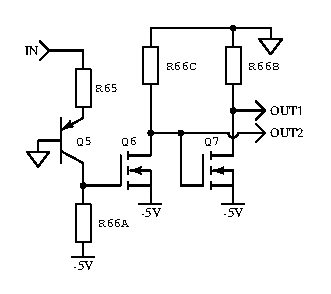
\includegraphics{gaasctl}
\caption{GaAs control circuit}
\label{fig:gaasctl}
\end{figure}

Figure~\ref{fig:gaasctl} is the control circuit for figure~\ref{fig:gaassw}.
When $0\;\mr{V}$ (a logic \emph{low}) is applied to the input from the
microcontroller, no current flows through \refdes{R65} or \refdes{R66A}.
This applies $-5\;\mr{V}$ to \refdes{Q6}. Because \refdes{Q6}'s source is
connected to the $-5\;\mr{V}$ rail instead of ground, the voltage between gate
and source ($V_{GS}$) is zero, and \refdes{Q6} is switched off.
This provides $0\;\mr{V}$ to one input of the GaAs switches. \refdes{Q7} acts
as an inverter, providing $-5\;\mr{V}$ to the other GaAs switch input. The
dual switches have their inputs connected opposite each other, so this
switches one of them \emph{on} and the other \emph{off}.

When $3.3\;\mr{V}$ (a logic \emph{high}) is applied to the input from the
microcontroller, about $1.6\;\mr{mA}$ flows through \refdes{R65}. This
saturates \refdes{Q5}, applying about $0.7\;\mr{V}$ to \refdes{Q6}. As above,
$V_{GS}$ is the difference between this and the $-5\;\mr{V}$ rail, or
$5.7\;\mr{V}$. \refdes{Q6} now switches on, and the two signals to the GaAs
switches swap places. This swaps the two switches, turning on the one that was
off, and turning off the one that was on.


\subsubsection{Buffer and Filter}
\subsubsection{Logarithmic Detector}


\section{Software Description}
\subsection{Signal Processing}
\subsubsection{Sampling}
\subsubsection{Null Search}
\subsubsection{Calibration}
\subsection{User Interface}



\end{multicols}

\newpage
\begin{landscape}
\chapter{Electrical parts}
\texttt{
\begin{longtable}{|l|l|l|l|l|}
\hline
\textbf{Reference} & \textbf{Manufacturer} & \textbf{Part Number} & \textbf{Line} & \textbf{Description} \\
\hline
\endhead
C1 &  &  & CAP MLCC 10nF 50V 10\% \ensuremath{\geq}X5R [0603] &  \\
\hline
C2 &  &  & CAP MLCC 10nF 50V 10\% \ensuremath{\geq}X5R [0603] &  \\
\hline
C3 &  &  & CAP MLCC 100nF 16V 10\% \ensuremath{\geq}X7R [0603] &  \\
\hline
C4 &  &  & CAP MLCC 10nF 50V 10\% \ensuremath{\geq}X5R [0603] &  \\
\hline
C5 &  &  & CAP MLCC 10\ensuremath{\mu}F 10V 10\% \ensuremath{\geq}X5R [0805] &  \\
\hline
C8 &  &  & CAP MLCC 100nF 16V 10\% \ensuremath{\geq}X7R [0603] &  \\
\hline
C9 &  &  & CAP MLCC 100nF 16V 10\% \ensuremath{\geq}X7R [0603] &  \\
\hline
C10 &  &  & CAP MLCC 100nF 16V 10\% \ensuremath{\geq}X7R [0603] &  \\
\hline
C11 &  &  & CAP MLCC 100nF 16V 10\% \ensuremath{\geq}X7R [0603] &  \\
\hline
C12 &  &  & CAP MLCC 100nF 16V 10\% \ensuremath{\geq}X7R [0603] &  \\
\hline
C13 &  &  & CAP MLCC 100nF 16V 10\% \ensuremath{\geq}X7R [0603] &  \\
\hline
C14 &  &  & CAP MLCC 15pF 50V 10\% C0G [0603] &  \\
\hline
C15 &  &  & CAP MLCC 15pF 50V 10\% C0G [0603] &  \\
\hline
C16 &  &  & CAP MLCC 100nF 16V 10\% \ensuremath{\geq}X7R [0603] &  \\
\hline
C17 &  &  & CAP MLCC 100nF 16V 10\% \ensuremath{\geq}X7R [0603] &  \\
\hline
C18 &  &  & CAP MLCC 100nF 16V 10\% \ensuremath{\geq}X7R [0603] &  \\
\hline
C19 &  &  & CAP MLCC 100nF 16V 10\% \ensuremath{\geq}X7R [0603] &  \\
\hline
C20 &  &  & CAP MLCC 100nF 16V 10\% \ensuremath{\geq}X7R [0603] &  \\
\hline
C21 &  &  & CAP MLCC 100nF 20V 10\% \ensuremath{\geq}X7R [0805] &  \\
\hline
C22 &  &  & CAP MLCC 100nF 16V 10\% \ensuremath{\geq}X7R [0603] &  \\
\hline
C23 &  &  & CAP MLCC 100nF 16V 10\% \ensuremath{\geq}X7R [0603] &  \\
\hline
C24 &  &  & CAP MLCC 100nF 20V 10\% \ensuremath{\geq}X7R [0805] &  \\
\hline
C25 &  &  & CAP MLCC 680pF 16V 5\% C0G [0603] &  \\
\hline
C26 &  &  & CAP MLCC 100nF 16V 10\% \ensuremath{\geq}X7R [0603] &  \\
\hline
C27 &  &  & CAP MLCC 100nF 16V 10\% \ensuremath{\geq}X7R [0603] &  \\
\hline
C28 &  &  & CAP MLCC 10\ensuremath{\mu}F 10V 10\% \ensuremath{\geq}X5R [0805] &  \\
\hline
C29 &  &  & CAP MLCC 10\ensuremath{\mu}F 10V 10\% \ensuremath{\geq}X5R [0805] &  \\
\hline
C30 &  &  & CAP MLCC 100nF 16V 10\% \ensuremath{\geq}X7R [0603] &  \\
\hline
C31 &  &  & CAP MLCC 100nF 16V 10\% \ensuremath{\geq}X7R [0603] &  \\
\hline
C32 &  &  & CAP MLCC 1nF 50V 10\% C0G [0603] &  \\
\hline
C33 &  &  & CAP MLCC 1nF 50V 10\% C0G [0603] &  \\
\hline
C34 &  &  & CAP MLCC 100nF 16V 10\% \ensuremath{\geq}X7R [0603] &  \\
\hline
C35 &  &  & CAP MLCC 100nF 16V 10\% \ensuremath{\geq}X7R [0603] &  \\
\hline
C36 &  &  & CAP MLCC 10\ensuremath{\mu}F 10V 10\% \ensuremath{\geq}X5R [0805] &  \\
\hline
C37 &  &  & CAP MLCC 10\ensuremath{\mu}F 10V 10\% \ensuremath{\geq}X5R [0805] &  \\
\hline
C38 &  &  & CAP MLCC 100nF 20V 10\% \ensuremath{\geq}X7R [0805] &  \\
\hline
C39 &  &  & CAP MLCC 100nF 20V 10\% \ensuremath{\geq}X7R [0805] &  \\
\hline
C40 &  &  & CAP MLCC 10\ensuremath{\mu}F 25V 10\% \ensuremath{\geq}X5R [1206] &  \\
\hline
C41 &  &  & CAP MLCC 10\ensuremath{\mu}F 25V 10\% \ensuremath{\geq}X5R [1206] &  \\
\hline
C43 & Murata & GRM1555C1H220GA01D & DIST DIGIKEY 490-6219-1-ND & CAP MLCC 22pF C0G [0402] \\
\hline
C44 & Murata & GRM1555C1H220GA01D & DIST DIGIKEY 490-6219-1-ND & CAP MLCC 22pF C0G [0402] \\
\hline
C45 & Samsung & CL10C1R5BB8NNNC & DIST DIGIKEY 1276-1656-1-ND & CAP MLCC 1.5pF C0G [0402] \\
\hline
C46 & Samsung & CL05C560JB5NNNC & DIST DIGIKEY 1276-1707-1-ND & CAP MLCC 56pF C0G [0402] \\
\hline
C47 & Samsung & CL05C4R7CB5NNNC & DIST DIGIKEY 1276-1703-1-ND & CAP MLCC 4.7pF C0G [0402] \\
\hline
C48 & Samsung & CL05C4R7CB5NNNC & DIST DIGIKEY 1276-1703-1-ND & CAP MLCC 4.7pF C0G [0402] \\
\hline
C49 & Samsung & CL05C560JB5NNNC & DIST DIGIKEY 1276-1707-1-ND & CAP MLCC 56pF C0G [0402] \\
\hline
C50 & Samsung & CL05C4R7CB5NNNC & DIST DIGIKEY 1276-1703-1-ND & CAP MLCC 4.7pF C0G [0402] \\
\hline
C51 & Murata & GRM1555C1H220GA01D & DIST DIGIKEY 490-6219-1-ND & CAP MLCC 22pF C0G [0402] \\
\hline
C52 & Murata & GRM1555C1H220GA01D & DIST DIGIKEY 490-6219-1-ND & CAP MLCC 22pF C0G [0402] \\
\hline
C53 &  &  & CAP MLCC 47\ensuremath{\mu}F 10V 20\% \ensuremath{\geq}X5R [1206] &  \\
\hline
C54 &  &  & CAP MLCC 1nF 50V 10\% C0G [0603] &  \\
\hline
C55 &  &  & CAP MLCC 100nF 20V 10\% \ensuremath{\geq}X7R [0805] &  \\
\hline
C56 &  &  & CAP MLCC 10nF 50V 10\% \ensuremath{\geq}X5R [0603] &  \\
\hline
C57 &  &  & CAP MLCC 1nF 50V 10\% C0G [0603] &  \\
\hline
C58 &  &  & CAP MLCC 1nF 50V 10\% C0G [0603] &  \\
\hline
C59 &  &  & CAP MLCC 100nF 16V 10\% \ensuremath{\geq}X7R [0603] &  \\
\hline
C60 & TDK & C1608C0G1H220F080AA & DIST DIGIKEY 445-5366-1-ND & CAP MLCC 22pF C0G [0402] \\
\hline
C61 & TDK & C1608C0G1H330F080AA & DIST DIGIKEY 445-7027-1-ND & CAP MLCC 33pF C0G [0402] \\
\hline
C62 & TDK & C1608C0G1H220F080AA & DIST DIGIKEY 445-5366-1-ND & CAP MLCC 22pF C0G [0402] \\
\hline
C63 &  &  & CAP MLCC 10nF 50V 10\% \ensuremath{\geq}X5R [0603] &  \\
\hline
C64 & TDK & C2012JB1H105K085AB & DIST DIGIKEY 445-11490-1-ND & CAP MLCC 1uF [0805] \\
\hline
C65 &  &  & CAP MLCC 10nF 50V 10\% \ensuremath{\geq}X5R [0603] &  \\
\hline
C66 & TDK & C2012JB1H105K085AB & DIST DIGIKEY 445-11490-1-ND & CAP MLCC 1uF [0805] \\
\hline
C67 &  &  & CAP MLCC 10nF 50V 10\% \ensuremath{\geq}X5R [0603] &  \\
\hline
C68 &  &  & CAP MLCC 100nF 16V 10\% \ensuremath{\geq}X7R [0603] &  \\
\hline
C69 &  &  & CAP MLCC 47\ensuremath{\mu}F 10V 20\% \ensuremath{\geq}X5R [1206] &  \\
\hline
C70 &  &  & CAP MLCC 220pF 16V 5\% C0G [0603] &  \\
\hline
C71 &  &  & CAP MLCC 330nF 50V 5\% \ensuremath{\geq}X7R [0603] &  \\
\hline
C72 &  &  & CAP MLCC 10nF 50V 10\% \ensuremath{\geq}X5R [0603] &  \\
\hline
C73 &  &  & CAP MLCC 100nF 20V 10\% \ensuremath{\geq}X7R [0805] &  \\
\hline
C74 &  &  & CAP MLCC 100nF 20V 10\% \ensuremath{\geq}X7R [0805] &  \\
\hline
C75 &  &  & CAP MLCC 10nF 50V 10\% \ensuremath{\geq}X5R [0603] &  \\
\hline
C76 & Panasonic & 16SVPC100M & DIST DIGIKEY P16468CT-ND & CAP ALU-POLY 100uF 16V \\
\hline
C77 & Panasonic & 16SVPC100M & DIST DIGIKEY P16468CT-ND & CAP ALU-POLY 100uF 16V \\
\hline
C78 &  &  & CAP MLCC 10nF 50V 10\% \ensuremath{\geq}X5R [0603] &  \\
\hline
C79 &  &  & CAP MLCC 10nF 50V 10\% \ensuremath{\geq}X5R [0603] &  \\
\hline
C80 &  &  & CAP MLCC 1nF 50V 10\% C0G [0603] &  \\
\hline
C81 &  &  & CAP MLCC 1nF 50V 10\% C0G [0603] &  \\
\hline
C82 & Panasonic & 16SVPC100M & DIST DIGIKEY P16468CT-ND & CAP ALU-POLY 100uF 16V \\
\hline
C83 & Panasonic & 16SVPC100M & DIST DIGIKEY P16468CT-ND & CAP ALU-POLY 100uF 16V \\
\hline
C84 &  &  & CAP MLCC 1\ensuremath{\mu}F 16V 10\% \ensuremath{\geq}X5R [1206] &  \\
\hline
C85 &  &  & CAP MLCC 1\ensuremath{\mu}F 16V 10\% \ensuremath{\geq}X5R [1206] &  \\
\hline
C86 &  &  & CAP MLCC 1\ensuremath{\mu}F 16V 10\% \ensuremath{\geq}X5R [1206] &  \\
\hline
C87 &  &  & CAP MLCC 1\ensuremath{\mu}F 16V 10\% \ensuremath{\geq}X5R [1206] &  \\
\hline
C88 &  &  & CAP MLCC 1\ensuremath{\mu}F 10V 10\% \ensuremath{\geq}X5R [0805] &  \\
\hline
C89 &  &  & CAP MLCC 1\ensuremath{\mu}F 16V 10\% \ensuremath{\geq}X5R [1206] &  \\
\hline
C90 &  &  & CAP MLCC 10\ensuremath{\mu}F 10V 10\% \ensuremath{\geq}X5R [0805] &  \\
\hline
C91 &  &  & CAP MLCC 10\ensuremath{\mu}F 10V 10\% \ensuremath{\geq}X5R [0805] &  \\
\hline
C92 &  &  & CAP MLCC 22\ensuremath{\mu}F 6V 10\% \ensuremath{\geq}X5R [0805] &  \\
\hline
C93 &  &  & CAP MLCC 1\ensuremath{\mu}F 10V 10\% \ensuremath{\geq}X5R [0805] &  \\
\hline
C97 &  &  & CAP MLCC 100nF 16V 10\% \ensuremath{\geq}X7R [0603] &  \\
\hline
C98 &  &  & CAP MLCC 100nF 16V 10\% \ensuremath{\geq}X7R [0603] &  \\
\hline
C100 &  &  & CAP MLCC 100nF 16V 10\% \ensuremath{\geq}X7R [0603] &  \\
\hline
C101 &  &  & CAP MLCC 100nF 16V 10\% \ensuremath{\geq}X7R [0603] &  \\
\hline
C102 &  &  & CAP MLCC 100nF 16V 10\% \ensuremath{\geq}X7R [0603] &  \\
\hline
C103 &  &  & CAP MLCC 100nF 16V 10\% \ensuremath{\geq}X7R [0603] &  \\
\hline
C104 &  &  & CAP MLCC 100nF 16V 10\% \ensuremath{\geq}X7R [0603] &  \\
\hline
C105 &  &  & CAP MLCC 100nF 16V 10\% \ensuremath{\geq}X7R [0603] &  \\
\hline
C106 &  &  & CAP MLCC 100nF 16V 10\% \ensuremath{\geq}X7R [0603] &  \\
\hline
C107 &  &  & CAP MLCC 10\ensuremath{\mu}F 10V 10\% \ensuremath{\geq}X5R [0805] &  \\
\hline
C108 &  &  & CAP MLCC 10\ensuremath{\mu}F 10V 10\% \ensuremath{\geq}X5R [0805] &  \\
\hline
C109 &  &  & CAP MLCC 1\ensuremath{\mu}F 10V 10\% \ensuremath{\geq}X5R [0805] &  \\
\hline
C110 &  &  & CAP MLCC 15pF 50V 10\% C0G [0603] &  \\
\hline
C111 &  &  & CAP MLCC 15pF 50V 10\% C0G [0603] &  \\
\hline
D3 &  & MMBD4148 & SEMI GENERIC MMBD4148 &  \\
\hline
D4 &  & MMBD4148 & SEMI GENERIC MMBD4148 &  \\
\hline
D5 &  & MMBD4148 & SEMI GENERIC MMBD4148 &  \\
\hline
D6 &  & MMBD4148 & SEMI GENERIC MMBD4148 &  \\
\hline
D7 &  & MBR0540 & SEMI GENERIC MBR0540 &  \\
\hline
D8 &  & MBR0540 & SEMI GENERIC MBR0540 &  \\
\hline
DS1 &  & LED RED [3mm] & SEMI GENERIC LED RED [3mm] &  \\
\hline
DS2 &  & LED RED [0603] & SEMI GENERIC LED RED [0603] &  \\
\hline
DS3 &  & LED RED [0603] & SEMI GENERIC LED RED [0603] &  \\
\hline
DS4 &  & LED RED [0603] & SEMI GENERIC LED RED [0603] &  \\
\hline
DS5 &  & LED RED [0603] & SEMI GENERIC LED RED [0603] &  \\
\hline
DS6 &  & LED RED [0603] & SEMI GENERIC LED RED [0603] &  \\
\hline
DS7 &  & LED RED [0603] & SEMI GENERIC LED RED [0603] &  \\
\hline
DS8 &  & LED RED [0603] & SEMI GENERIC LED RED [0603] &  \\
\hline
DS9 &  & LED RED [0603] & SEMI GENERIC LED RED [0603] &  \\
\hline
DS10 &  & LED RED [0603] & SEMI GENERIC LED RED [0603] &  \\
\hline
DS11 &  & LED RED [0603] & SEMI GENERIC LED RED [0603] &  \\
\hline
DZ1 & ONSEMI & 1SMA5914BT3G & SEMI ONSEMI 1SMA5914BT3G &  \\
\hline
DZ2 & LITTELFUSE & SP0503BAHT & SEMI LITTELFUSE SP0503BAHT &  \\
\hline
DZ3 & ONSEMI & ESD9L5.0ST5G & SEMI ONSEMI ESD9L5.0ST5G &  \\
\hline
DZ4 & ONSEMI & ESD9L5.0ST5G & SEMI ONSEMI ESD9L5.0ST5G &  \\
\hline
DZ5 &  & BZX84C2V7 & SEMI GENERIC BZX84C2V7 &  \\
\hline
DZ6 &  & BZX84C2V7 & SEMI GENERIC BZX84C2V7 &  \\
\hline
DZ7 & ONSEMI & ESD9L5.0ST5G & SEMI ONSEMI ESD9L5.0ST5G &  \\
\hline
DZ8 & ONSEMI & ESD9L5.0ST5G & SEMI ONSEMI ESD9L5.0ST5G &  \\
\hline
DZ9 &  & BZX84C3V9 & SEMI GENERIC BZX84C3V9 &  \\
\hline
DZ10 &  & BZX84C10 & SEMI GENERIC BZX84C10 &  \\
\hline
E1 & Laird & HZ0805B222R-10 & DIST DIGIKEY 240-2562-1-ND & FERRITE CHIP 2.2k @ 100MHz [0805] \\
\hline
E2 & Laird & HZ0805B222R-10 & DIST DIGIKEY 240-2562-1-ND & FERRITE CHIP 2.2k @ 100MHz [0805] \\
\hline
E5 & Bourns & MZ1608-102Y & DIST DIGIKEY MZ1608-102YCT-ND & FERRITE CHIP 1k @ 100MHz [0603] \\
\hline
J1 & CUI & PJ-037A & DIST DIGIKEY CP-037A-ND & CONN BARREL 2x6.5MM \\
\hline
J2 & TE & 5-1814400-1 & DIST DIGIKEY A97593-ND & CONN SMA RIGHTANGLE FEMALE \\
\hline
J3 & TE & 5-1814400-1 & DIST DIGIKEY A97593-ND & CONN SMA RIGHTANGLE FEMALE \\
\hline
J4 & TE & 5-1814400-1 & DIST DIGIKEY A97593-ND & CONN SMA RIGHTANGLE FEMALE \\
\hline
J6 & FCI & 10118194-0001LF & DIST DIGIKEY 609-4618-1-ND & CONN USB MICRO-B FEMALE \\
\hline
J8 & ONSHORE & 302-S201 & DIST DIGIKEY ED10524-ND & HEADER 2x10 100MIL SHROUDED \\
\hline
L1 & Samsung & CIH05T56NJNC & DIST DIGIKEY 1276-6281-1-ND & IND CHIP 56nH \\
\hline
L2 & Samsung & CIH05T47NJNC & DIST DIGIKEY 1276-6280-1-ND & IND CHIP 47nH \\
\hline
L3 & Samsung & CIH05T47NJNC & DIST DIGIKEY 1276-6280-1-ND & IND CHIP 47nH \\
\hline
L4 & Panasonic & ELJ-RF39NGFB & DIST DIGIKEY PCD1917CT-ND & IND CHIP 39nH \\
\hline
L5 & Panasonic & ELJ-RF39NGFB & DIST DIGIKEY PCD1917CT-ND & IND CHIP 39nH \\
\hline
L6 & Bourns & RLB0914-221KL & DIST DIGIKEY RLB0914-221KL-ND & IND WOUND 220uH 700mA \\
\hline
L7 & Bourns & RLB0914-221KL & DIST DIGIKEY RLB0914-221KL-ND & IND WOUND 220uH 700mA \\
\hline
L8 & TDK & MLZ2012M4R7HT000 & DIST DIGIKEY 445-8659-1-ND & IND CHIP 4.7uH 300mA [0805] \\
\hline
L9 & TDK & MLZ2012M4R7HT000 & DIST DIGIKEY 445-8659-1-ND & IND CHIP 4.7uH 300mA [0805] \\
\hline
L10 & TDK & MLZ2012M4R7HT000 & DIST DIGIKEY 445-8659-1-ND & IND CHIP 4.7uH 300mA [0805] \\
\hline
MP5 & Laird & BMI-S-203F; BMI-S-203-C & DIST DIGIKEY 903-1052-1-ND; & RF SHIELD TWO-PIECE \\
\hline
Q1 & IRF & IRLML6402 & SEMI IRF IRLML6402 &  \\
\hline
Q2 &  & MMBT3906 & SEMI GENERIC MMBT3906 &  \\
\hline
Q3 &  & 2N7002 & SEMI GENERIC 2N7002 &  \\
\hline
Q4 &  & 2N7002 & SEMI GENERIC 2N7002 &  \\
\hline
Q5 &  & MMBT3906 & SEMI GENERIC MMBT3906 &  \\
\hline
Q6 &  & 2N7002 & SEMI GENERIC 2N7002 &  \\
\hline
Q7 &  & 2N7002 & SEMI GENERIC 2N7002 &  \\
\hline
Q8 &  & MMBT3904 & SEMI GENERIC MMBT3904 &  \\
\hline
Q9 & NXP & BFR540 & SEMI NXP BFR540 &  \\
\hline
Q10 & NXP & BFR540 & SEMI NXP BFR540 &  \\
\hline
Q11 &  & MMBT3904 & SEMI GENERIC MMBT3904 &  \\
\hline
Q12 &  & MMBT3906 & SEMI GENERIC MMBT3906 &  \\
\hline
Q13 & IRF & IRLML6402 & SEMI IRF IRLML6402 &  \\
\hline
Q14 & AOS & AOD417 & SEMI AOS AOD417 &  \\
\hline
Q15 &  & MMBT3904 & SEMI GENERIC MMBT3904 &  \\
\hline
Q16 &  & MMBT3904 & SEMI GENERIC MMBT3904 &  \\
\hline
Q17 &  & PZT2907A & SEMI GENERIC PZT2907A &  \\
\hline
Q18 &  & PZT2907A & SEMI GENERIC PZT2907A &  \\
\hline
Q19 &  & MMBT3904 & SEMI GENERIC MMBT3904 &  \\
\hline
Q20 &  & MMBT3904 & SEMI GENERIC MMBT3904 &  \\
\hline
R1 &  &  & RES SMD 3.3k 5\% [0603] &  \\
\hline
R2 &  &  & RES SMD 1.6k 1\% [0603] &  \\
\hline
R3 &  &  & RES SMD 1.6k 1\% [0603] &  \\
\hline
R4 &  &  & RES SMD 3.3k 5\% [0603] &  \\
\hline
R5 &  &  & RES SMD 1.6k 1\% [0603] &  \\
\hline
R6 &  &  & RES SMD 1.6k 1\% [0603] &  \\
\hline
R7 &  &  & RES SMD 1.6k 1\% [0603] &  \\
\hline
R8 &  &  & RES SMD 3.3k 5\% [0603] &  \\
\hline
R9 &  &  & RES SMD 3.3k 5\% [0603] &  \\
\hline
R10 & Bel Fuse & 0ZCJ0005FF2E & DIST DIGIKEY 507-1793-1-ND & PPTC 50mA/150mA 60V [1206] \\
\hline
R11 & Bel Fuse & 0ZCJ0005FF2E & DIST DIGIKEY 507-1793-1-ND & PPTC 50mA/150mA 60V [1206] \\
\hline
R12 & Bel Fuse & 0ZCJ0005FF2E & DIST DIGIKEY 507-1793-1-ND & PPTC 50mA/150mA 60V [1206] \\
\hline
R13 &  &  & RES SMD 1M 5\% [0603] &  \\
\hline
R14 &  &  & RES SMD 30 1\% [0603] &  \\
\hline
R15 &  &  & RES SMD 30 1\% [0603] &  \\
\hline
R16 &  &  & RES SMD 1M 5\% [0603] &  \\
\hline
R17 &  &  & RES SMD 1M 5\% [0603] &  \\
\hline
R18 &  &  & RES SMD 49.9 1\% [0603] &  \\
\hline
R19 &  &  & RES SMD 1.91k 1\% [0603] &  \\
\hline
R21 &  &  & RES SMD 49.9 1\% [0603] &  \\
\hline
R22 &  &  & RES SMD 49.9 1\% [0603] &  \\
\hline
R23 &  &  & RES SMD 49.9 1\% [0603] &  \\
\hline
R24 &  &  & RES SMD 53.6 1\% [0603] &  \\
\hline
R25 &  &  & RES SMD 53.6 1\% [0603] &  \\
\hline
R26 &  &  & RES SMD 53.6 1\% [0603] &  \\
\hline
R27 &  &  & RES SMD 53.6 1\% [0603] &  \\
\hline
R28 &  &  & RES SMD 360 1\% [0603] &  \\
\hline
R29 &  &  & RES SMD 360 1\% [0603] &  \\
\hline
R30 &  &  & RES SMD 360 1\% [0603] &  \\
\hline
R31 &  &  & RES SMD 360 1\% [0603] &  \\
\hline
R32 &  &  & RES SMD 360 1\% [0603] &  \\
\hline
R33 &  &  & RES SMD 360 1\% [0603] &  \\
\hline
R34 &  &  & RES SMD 360 1\% [0603] &  \\
\hline
R35 &  &  & RES SMD 360 1\% [0603] &  \\
\hline
R36 &  &  & RES SMD 1.91k 1\% [0603] &  \\
\hline
R37 &  &  & RES SMD 1.91k 1\% [0603] &  \\
\hline
R38 &  &  & RES SMD 49.9 1\% [0603] &  \\
\hline
R39 &  &  & RES SMD 49.9 1\% [0603] &  \\
\hline
R40 &  &  & RES SMD 1.6k 1\% [0603] &  \\
\hline
R41 & Yageo & YC164-JR-0710KL & DIST DIGIKEY YC164J-10KCT-ND & RESPACK SMD 10k 5\% [4x0603] \\
\hline
R42 &  &  & RES SMD 200 1\% [0603] &  \\
\hline
R43 &  &  & RES SMD 200 1\% [0603] &  \\
\hline
R45 &  &  & RES SMD 30 1\% [0603] &  \\
\hline
R46 &  &  & RES SMD 49.9 1\% [0603] &  \\
\hline
R47 &  &  & RES SMD 150 1\% [0603] &  \\
\hline
R48 &  &  & RES SMD 750 1\% [0603] &  \\
\hline
R49 &  &  & RES SMD 150 1\% [0603] &  \\
\hline
R50 &  &  & RES SMD 33 1\% [0603] &  \\
\hline
R51 &  &  & RES SMD 33 1\% [0603] &  \\
\hline
R52 &  &  & RES SMD 33 1\% [0603] &  \\
\hline
R53 &  &  & RES SMD 33 1\% [0603] &  \\
\hline
R54 &  &  & RES SMD 33 1\% [0603] &  \\
\hline
R55 &  &  & RES SMD 33 1\% [0603] &  \\
\hline
R56 &  &  & RES SMD 49.9 1\% [0603] &  \\
\hline
R57 &  &  & RES SMD 1.6k 1\% [0603] &  \\
\hline
R58 &  &  & RES SMD 1.6k 1\% [0603] &  \\
\hline
R59 &  &  & RES SMD 3.3 10\% [0603] &  \\
\hline
R60 &  &  & RES SMD 750 1\% [0603] &  \\
\hline
R61 &  &  & RES SMD 750 1\% [0603] &  \\
\hline
R62 &  &  & RES SMD 1.6k 1\% [0603] &  \\
\hline
R63 &  &  & RES SMD 1.6k 1\% [0603] &  \\
\hline
R64 &  &  & RES SMD 3.3 10\% [0603] &  \\
\hline
R65 &  &  & RES SMD 1.6k 1\% [0603] &  \\
\hline
R66 & Yageo & YC164-JR-0710KL & DIST DIGIKEY YC164J-10KCT-ND & RESPACK SMD 10k 5\% [4x0603] \\
\hline
R67 &  &  & RES SMD 200 1\% [0603] &  \\
\hline
R68 &  &  & RES SMD 200 1\% [0603] &  \\
\hline
R69 &  &  & RES SMD 200 1\% [0603] &  \\
\hline
R70 &  &  & RES SMD 200 1\% [0603] &  \\
\hline
R71 &  &  & RES SMD 200 1\% [0603] &  \\
\hline
R72 &  &  & RES SMD 200 1\% [0603] &  \\
\hline
R73 &  &  & RES SMD 1.6k 1\% [0603] &  \\
\hline
R74 &  &  & RES SMD 30 1\% [0603] &  \\
\hline
R75 &  &  & RES SMD 100 1\% [0603] &  \\
\hline
R76 &  &  & RES SMD 100 1\% [0603] &  \\
\hline
R77 &  &  & RES SMD 100 1\% [0603] &  \\
\hline
R78 &  &  & RES SMD 3.3k 5\% [0603] &  \\
\hline
R79 &  &  & RES SMD 53.6 1\% [0603] &  \\
\hline
R80 &  &  & RES SMD 49.9 1\% [0603] &  \\
\hline
R81 & BelFuse & 0ZCJ0035AF2E & DIST DIGIKEY 507-1801-1-ND & PPTC 350mA/750mA 30V [1206] \\
\hline
R82 &  &  & RES SMD 3.3k 5\% [0603] &  \\
\hline
R83 & Yageo & YC164-JR-0710KL & DIST DIGIKEY YC164J-10KCT-ND & RESPACK SMD 10k 5\% [4x0603] \\
\hline
R84 & Yageo & YC164-JR-0710KL & DIST DIGIKEY YC164J-10KCT-ND & RESPACK SMD 10k 5\% [4x0603] \\
\hline
R85 & Yageo & YC164-JR-0710KL & DIST DIGIKEY YC164J-10KCT-ND & RESPACK SMD 10k 5\% [4x0603] \\
\hline
R86 &  &  & RES SMD 3.3k 5\% [0603] &  \\
\hline
R87 &  &  & RES SMD 1M 5\% [0603] &  \\
\hline
R88 &  &  & RES SMD 1M 5\% [0603] &  \\
\hline
R89 &  &  & RES SMD 3.3k 5\% [0603] &  \\
\hline
R90 &  &  & RES SMD 3.3k 5\% [0603] &  \\
\hline
R91 &  &  & RES SMD 1.6k 1\% [0603] &  \\
\hline
R92 &  &  & RES SMD 750 1\% [0603] &  \\
\hline
R93 &  &  & RES SMD 1.6k 1\% [0603] &  \\
\hline
R94 &  &  & RES SMD 750 1\% [0603] &  \\
\hline
R95 &  &  & RES SMD 1 5\% [1210] &  \\
\hline
R96 &  &  & RES SMD 1 5\% [1210] &  \\
\hline
R97 & BelFuse & 0ZCJ0010FF2E & DIST DIGIKEY 507-1794-1-ND & PPTC 100mA/250mA 60V [1206] \\
\hline
R98 &  &  & RES SMD 3.3 10\% [0603] &  \\
\hline
R99 &  &  & RES SMD 3.3 10\% [0603] &  \\
\hline
R102 &  &  & RES SMD 3.3k 5\% [0603] &  \\
\hline
R103 &  &  & RES SMD 3.3k 5\% [0603] &  \\
\hline
R104 &  &  & RES SMD 3.3k 5\% [0603] &  \\
\hline
R105 &  &  & RES SMD 3.3k 5\% [0603] &  \\
\hline
R106 &  &  & RES SMD 1k 5\% [0603] &  \\
\hline
R107 &  &  & RES SMD 1k 5\% [0603] &  \\
\hline
R108 &  &  & RES SMD 1k 5\% [0603] &  \\
\hline
R109 &  &  & RES SMD 1k 5\% [0603] &  \\
\hline
R110 &  &  & RES SMD 200 1\% [0603] &  \\
\hline
R111 &  &  & RES SMD 3.3k 5\% [0603] &  \\
\hline
R112 &  &  & RES SMD 200 1\% [0603] &  \\
\hline
R113 &  &  & RES SMD 200 1\% [0603] &  \\
\hline
R114 &  &  & RES SMD 200 1\% [0603] &  \\
\hline
R115 &  &  & RES SMD 200 1\% [0603] &  \\
\hline
R116 &  &  & RES SMD 200 1\% [0603] &  \\
\hline
R117 &  &  & RES SMD 360 1\% [0603] &  \\
\hline
U2 & TI & LMH6714MF & IC TI LMH6714MF &  \\
\hline
U3 & ADI & AD9958BCPZ & IC ADI AD9958BCPZ &  \\
\hline
U4 & TI & LMH6714MF & IC TI LMH6714MF &  \\
\hline
U5 & ADI & AD8000YRDZ & IC ADI AD8000YRDZ &  \\
\hline
U6 & TI & THS3001IDGN & IC TI THS3001IDGN &  \\
\hline
U7 & MACOM & MAADSS0008 & IC MACOM MAADSS0008 &  \\
\hline
U8 & MACOM & MASWSS0162 & IC MACOM MASWSS0162 &  \\
\hline
U9 & MACOM & MASWSS0162 & IC MACOM MASWSS0162 &  \\
\hline
U10 & ADI & AD8310ARMZ & IC ADI AD8310ARMZ &  \\
\hline
U11 & TI & TL431AIDBZ & IC TI TL431AIDBZ &  \\
\hline
U12 &  & LM393M & IC GENERIC LM393M &  \\
\hline
U13 & ST & L78M05CDT & IC ST L78M05CDT &  \\
\hline
U14 & ONSEMI & MC79M05CDTG & IC ONSEMI MC79M05CDTG &  \\
\hline
U15 & DIODES & AZ1117CH-1.8TRG1 & IC DIODES AZ1117CH-1.8TRG1 &  \\
\hline
U16 & MICROCHIP & MCP1700T-3302E/TT & IC MICROCHIP MCP1700T-3302E/TT &  \\
\hline
U18 & ATMEL & ATSAM4S16CA-AU & IC ATMEL ATSAM4S16CA-AU &  \\
\hline
X1 & TXC & 9C-25.000MEEJ-T & DIST DIGIKEY 887-1283-1-ND & CRYSTAL 25MHz 18pF 10PPM \\
\hline
X2 & Abracon & ABLS-12.000MHZ-B4-T & DIST DIGIKEY 535-10218-1-ND & CRYSTAL 12MHz 18pF \\
\hline
\end{longtable}

}
\end{landscape}

\newpage
\chapter{Full schematics}
The following pages contain schematics exported directly from the CAD software.
While they are documented, it is intended that readers will first familiarize
themselves with the workings of the circuits by reading through the
\hyperref[chap:too]{Theory of Operation}.
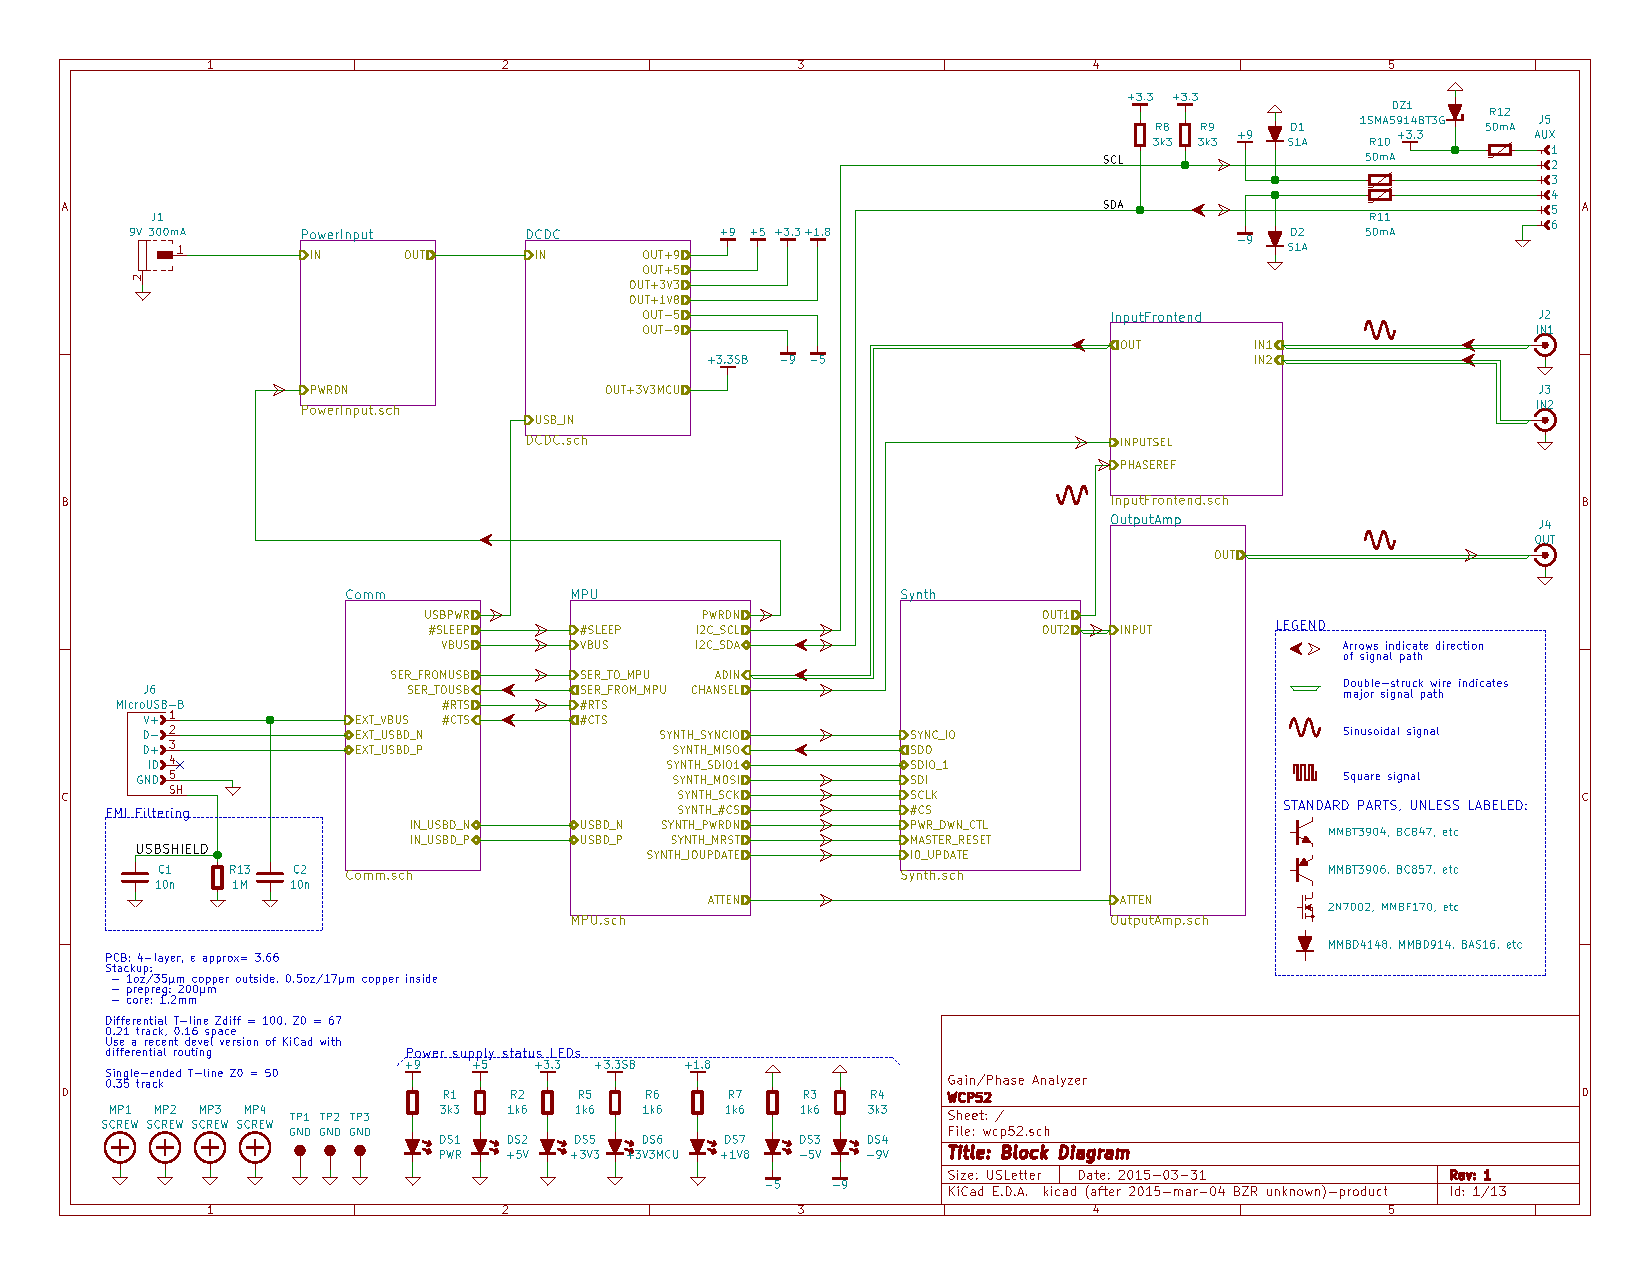
\includepdf[landscape=true,pages=-,link]{schematic.pdf}
\newpage
\begin{thebibliography}{9}

\bibitem{aod417}
Alpha \& Omega Semiconductor, ``AOD417 P-Channel Enhancement Mode Field Effect Transistor,''
AOD417 datasheet, 2008. \url{http://aosmd.com/pdfs/datasheet/AOD417.pdf}

\bibitem{tranckts-sawtooth}
S. W. Amos and M. James, ``Sawtooth generators,'' in
\emph{Principles of Transistor Circuits}, 9th ed. Oxford: Newnes, 2003, ch. 14, pp. 281--292.

\bibitem{az1117c}
Diodes Incorporated, ``Low Dropout Linear Regulator,'' AZ1117C datasheet,
October 2014 [Revision 3--2].
\url{http://www.diodes.com/datasheets/AZ1117C.pdf}

\bibitem{aoe-vreg}
P. Horowitz and W. Hill, ``Voltage regulators and power circuits,'' in
\emph{The Art of Electronics}, 2nd ed. Cambridge: Cambridge, 1989, ch. 6, pp. 307--389.

\bibitem{mcp1700}
Microchip Technology, ``Low Quiescent Current LDO,'' MCP1700 datasheet,
October 2013 [Revision C].
\url{http://ww1.microchip.com/downloads/en/DeviceDoc/20001826C.pdf}

\bibitem{mc79m00}
ON Semiconductor, ``500 mA Negative Voltage Regulators,'' MC79M00 series datasheet,
July 2013 [Revision 15].
\url{http://www.onsemi.com/pub_link/Collateral/MC79M00-D.PDF}.

\bibitem{l78m05}
STMicroelectronics, ``Precision 500 mA regulators,'' L78M datasheet, June 2014 [Revision 20].
\url{http://www.st.com/web/en/resource/technical/document/datasheet/CD00000447.pdf}

\bibitem{tl431}
Texas Instruments, ``TL43xx Precision Programmable Reference,''
TL431 datasheet, Aug. 2004 [Revised Jan. 2015]. \url{http://www.ti.com/lit/ds/symlink/tl431.pdf}

\bibitem{buckinv}
J. Tucker, ``Using a buck converter in an inverting buck-boost topology,''
\emph{Analog Applications Journal}, Texas Instruments, fourth quarter 2007, pp. 16--19.
\url{http://www.ti.com/lit/an/slyt286/slyt286.pdf}
\end{thebibliography}


\end{document}
